\chapter{Instruction Level Parallelism (ILP)}

\section{Introduzione}

\dfn{Instruction Level Parallelism (ILP)}{
I processori che tratteremo sono pipelined e superscalari: 

\begin{enumerate}
  \item Eseguono le istruzioni in pipeline.
  \item Avviano all'esecuzione in parallelo più istruzioni per ciclo di clock.
\end{enumerate} 
} 

\subsubsection{Per implementare ILP:} 

\begin{enumerate}
  \item Deve essere disponibile un numero sufficiente di unità funzionali. 
  \item Deve essere possibile prelevare dalla instruction memory più istruzioni e 
    dalla data memory più operandi (le cache servono a facilitare questo). 
  \item Deve essere possibile indirizzare in parallelo più registri 
    della CPU e deve essere possibile leggere/scrivere i registri usati  dalle diverse istruzioni   in esecuzione nello stesso ciclo di clock.
\end{enumerate}

\subsection{Aumentare la Frequenza del Clock della CPU} 

Ciò significa un ciclo di clock più corto con una divisione in un maggiore numero di fasi. Se aumenta il numero di fasi (\fancyglitter{profondità}) allora ci saranno più istruzioni in esecuzione contemporaneamente. 

\nt{Questa relazione tra numero di fasi e ciclo di clock fu pesantemente sfruttata nel pentium IV in cui si sfioravano i 4 GHz con pipeline di quasi 30 stadi.} 

\subsubsection{Tuttavia non è possibile sfruttare all'infinito questa tecnica perché:}

\begin{enumerate}
  \item Maggiore è il numero di fasi, maggiore è la complessità della pipeline e quindi la sua control unit. 
  \item Frequenze di clock maggiori producono interferenze tra le piste, consumi e conseguenti problemi di dissipazione del calore.
\end{enumerate}

\dfn{Overclocking}{ 
Il progettista di una CPU non tara il ciclo di clock sulla durata esatta del tempo necessario all'impulso elettrico per attraversare una parte del datapath, ma lo rende un po' più lungo. Su quella differenza gli smanettoni possono "giocare" per 
aumentare le prestazioni della CPU.
}

\begin{figure}[!h]
    \centering
    
\includegraphics[scale=0.4]{02-ILP/lain.png}
    \caption{Io che faccio overclock del case.}
\end{figure}

\subsection{Multiple Issue}

\dfn{Multiple Issue}{ 
 Il Multiple Issue consiste nell'aumentare il numero di istruzioni eseguite in parallelo a ogni ciclo di clock. 
 Le architetture che  implementano un multiple issue dinamico vengono dette \newfancyglitter{superscalari}.
}

\nt{ 
  Si può vedere il multiple issue come più pipeline che eseguono istruzioni in parallelo. 
} 

\clm{}{}{ 
\begin{itemize}
  \item In un'architettura pipelined senza multiple issue, in assenza di stall, il CPI è uguale a 1. 
  \item Introducendo il multiple issue il CPI diventa minore di 1 (più istruzioni per ciclo di clock). 
  \item Tuttavia, nel caso reale, anche implementando multiple issue si ha un CPI maggiore di 1 per via dei problemi strutturali sui dati e sul controllo.
\end{itemize}
}

Per implementare il multiple issue è necessario determinare quali e quante istruzioni possono 
essere avviate all'esecuzione in un dato ciclo di clock. La ricerca è effettuata tra le istruzioni \fancyglitter{in attesa} di essere eseguite e ci sono limiti a quante istruzioni possono essere
analizzate contemporaneamente. Una volta individuate vengono impacchettate in un \fancyglitter{issue packet} e avviate all'esecuzione nello stesso \fancyglitter{issue slot} (ciclo di clock).
I processori multiple issue si possono dividere in due categorie a seconda di come e quando vengono risolti questi problemi: 

\begin{itemize}
  \item \fancyglitter{Multiple Issue statico:} è il compilatore, a livello software, a decidere quali istruzioni mandare in esecuzione in parallelo. Quando il processore preleva dalla Instruction Memory un pacchetto di istruzioni sa già che potrà eseguirle in parallelo. Il numero di istruzioni per pacchetto è stabilito a priori, nella fase di progettazione del processore (adottato principalmente da processori embedded). 
\item \fancyglitter{Multiple Issue dinamico:} è la CPU stessa che analizza, a runtime, le istruzioni e decide quali mandare in esecuzione in parallelo nello stesso ciclo di clock. C'è un limite al numero massimo di istruzioni analizzabile, di solito 3 o 4 (adottato principalmente da processori moderni dei PC).
\end{itemize} 

\nt{ILP dinamico e ILP statico non sono interamente distinti. I processori di una categoria adottano sempre anche qualche tecnica dell'altra.}

\section{ILP Dinamico}

Per avvicinare una pipeline alle sue prestazioni ideali si utilizzano tre tecniche:

\begin{enumerate}
  \item \fancyglitter{Scheduling dinamico della pipeline}. 
  \item \fancyglitter{Branch prediction}. 
  \item \fancyglitter{Speculazione hardware}.
\end{enumerate}

\subsection{Scheduling Dinamico, Branch Prediction e Speculazione Hardware}

Consideriamo questo programma  e supponiamo che 100(R2) non si trovi nella cache. 

\begin{center} 
  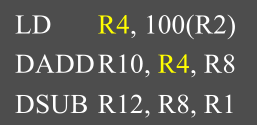
\includegraphics[scale=0.5]{02-ILP/es.png}
\end{center} 

L'esecuzione della DADD dipende dalla LD, ma in una pipeline le istruzioni procedono una dopo l'altra. Però la DSUB rimane bloccata anche se non sta aspettando alcun valore dalla LD e dalla DADD

\dfn{Scheduling dinamico della pipeline}{ 
Nello scheduling dinamico della pipeline l'ordine con cui le istruzioni vengono avviate alla fase EX può essere diverso dall'ordine in cui sono state prelevate dalla memoria di istruzioni. 
}

\nt{ 
  Nell'esempio precedente la DADD deve aspettare la LD, ma la DSUB può essere eseguita indipendentemente. 
}

\cor{Out-of-order}{ 
  Lo scheduling dinamico della pipeline permette sia l'esecuzione out-of-order che il completamento out-of-order. Le istruzioni possono eseguire la fase WB in un ordine diverso da quello in cui compaiono nel programma. 
}

In un sistema che implementa ILP statico è il compilatore ad accorgersicdi una situazione di potenziale stallo e genera un codice oggetto in cui la DSUB e posta prima della LD. 

\dfn{Branch Prediction Dinamica}{ 
Per ogni salto condizionato si memorizza l'esito della sua esecuzione. Se lo stesso salto viene eseguito di nuovo si utilizza il risultato precedente per fare una predizione.
}

\nt{ Utile con i cicli, soprattutto se vengono eseguiti molte volte. }

\dfn{Speculazione Hardware}{ 
Estensione della branch prediction: si presuppone che le istruzioni vengano eseguite dopo un salto. Se la predizione è corretta si è fatto del lavoro in anticipo, altrimenti si devono cancellare gli effetti di questa speculazione. 
}

\subsection{I Problemi di Fondo}

\subsubsection{Le istruzioni dipendono l'una dall altre.}

\dfn{True Data Dependence}{Le istruzioni hanno bisogno di argomenti, ma quegli argomenti possono essere il risultato di altre istruzioni.}

\cor{Istruzioni Indipendenti}{ 
  Due istruzioni sono \fancyglitter{indipendenti} tra loro se possono essere eseguite simultaneamente e/o in qualsiasi ordine a condizione che ci siano risorse sufficienti. 
} 

\cor{Istruzioni Dipendenti}{ 
  Due istruzioni sono \fancyglitter{dipendenti} se non possono essere eseguite in modo sovrapposto e quindi devono essere eseguite in ordine.
}

\subsubsection{Le istruzioni devono riutilizzare i registri.}

Dato che il numero di registri è limitato alcuni registri devono essere riutilizzati terminata la loro funzione. 

\begin{figure}[!h]
    \centering
    
\includegraphics[scale=0.4]{02-ILP/namedep.png}
    \caption{Name Dependence.}
\end{figure}

\nt{In questo caso non c'è un passaggio di valori tra la PRINT e la LOAD, ma finché la PRINT non è stata completata il registro R7 non può essere riutilizzato.}

\dfn{Name Dependence}{ 
Stessi registri vengono utilizzati da istruzione che altrimenti sarebbero indipendenti tra di loro.
}

Data l'istruzione $i$ che precede l'istruzione $j$ si possono avere: 

\begin{itemize}
  \item \fancyglitter{Antidipendenza} se $i$ legge in un registro che $j$ deve scrivere. L'istruzione $i$ deve aver tempo di leggere il registro prima che venga sovrascritto da $j$, altrimenti legge un valore sbagliato.
  \item \fancyglitter{Dipendenza in output} se $i$ e $j$ scrivono nello stesso registro. Il valore finale deve essere quello di $j$.
\end{itemize}

\ex{}{ 
\begin{center} 
  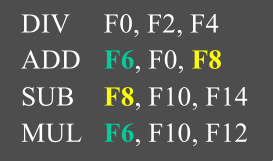
\includegraphics[scale=0.5]{02-ILP/dip.png}
\end{center} 

Tra ADD e SUB si ha un antidipedenza, mentre tra ADD e MUL si ha una dipendenza in output.
}

\clm{}{}{ 
\begin{itemize}
  \item La dipendenza sui nomi non è una vera dipendenza perché non ci sono valori trasmessi tra le istruzioni. 
  \item Le istruzioni coinvolte in una dipendenza sui nomi potrebbero essere eseguite in parallelo se il nome del registro usato venisse cambiato. 
  \item La ridenominazione può essere fatta staticamente dal compilatore o dinamicamente dalla CPU mentre esegue le istruzioni.
\end{itemize}

}

\ex{}{ 
\begin{center} 
  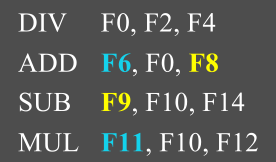
\includegraphics[scale=0.5]{02-ILP/dip2.png}
\end{center} 

}

\nt{ 
  Una tecnica alternativa è quella di utilizzare registri aggiuntivi \fancyglitter{nascosti}.
}

\subsection{L'Approccio di Tomasulo}

Nel 1967, Robert Tomasulo (ricercatore dell'IBM), sviluppo una tecnica per lo scheduling dinamico della pipeline: 

\begin{itemize}
  \item Per minimizzare le dipendenze sui dati tiene traccia di quando gli operandi delle istruzioni sono disponibili, indipendentemente dall'ordine in cui le istruzioni sono entrate nella CPU. 
  \item Per minimizzare le dipendenze sui nomi un insieme di registri interni alla CPU, invisibili a livello ISA viene usato per implementare la ridenominazione dei registri.
\end{itemize}

\begin{figure}[!h]
    \centering
    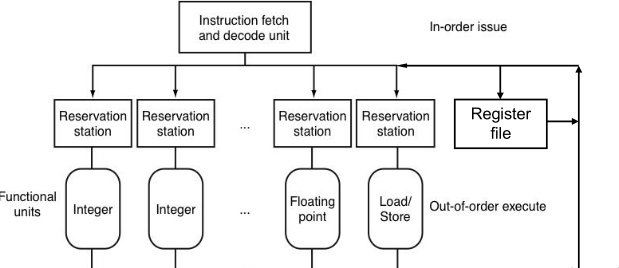
\includegraphics[scale=0.6]{02-ILP/Schema di Tomasulo.png}
    \caption{Lo schema di Tomasulo.}
\end{figure}

\cor{Reservation Station}{
  Le \fancyglitter{stazioni di prenotazione} servono da stallo per le istruzioni che verranno eseguite quando gli operandi saranno disponibili.

}

\begin{figure}[!h]
    \centering
    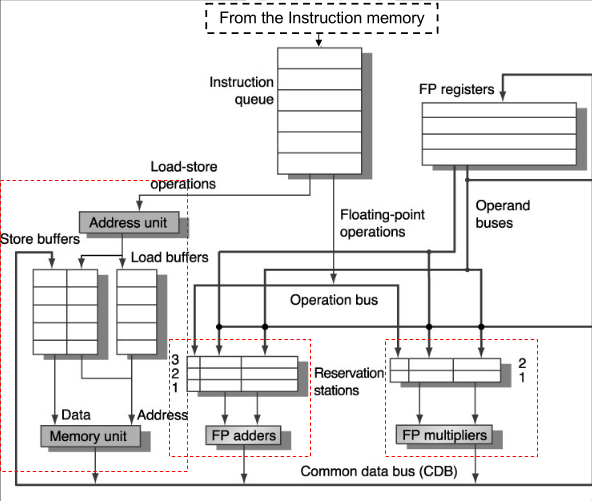
\includegraphics[scale=0.5]{02-ILP/Schema di Tomasulo 2.png}
    \caption{Sezione dello schema di Tomasulo che si occupa delle operazioni floating point.}
\end{figure}

Ogni stazione di prenotazione è fatta da una o più entry. Quando un'entry contiene un'istruzione,
per ogni operando dell'istruzione l'entry memorizza anche: 

\begin{itemize}
  \item Se già disponibile: il valore dell'operando stesso. 
  \item Se l'operando non è ancora stato calcolato: l'identificativo della entry della stazione di prenotazione che contiene l'istruzione che dovrà produrre il valore dell'operando mancante.
\end{itemize}

\cor{Common Data Bus}{ 
Il common data bus permette di trasferire in parallelo il risultato prodotto in output da una unità funzionale a tutte le stazioni di prenotazione che lo stanno aspettando e al register file.
}

\paragraph{Nello schema di Tomasulo l'esecuzione di un'istruzione è divisa in tre macropassi:} 

\begin{enumerate}
  \item \fancyglitter{Issue:} prelievo, decodifica e inserimento dell'istruzione in una entry della stazione di prenotazione associata all'unità funzionale che dovrà eseguire quell'istruzione. Se non ci sono entry vuote disponibili si ha stall della pipeline. Se gli operandi dell'istruzione sono disponibili nel register file o in qualche altra stazione di prenotazione vengono prelevati e mandati nella entry in cui è stata messa l'istruzione. 
    Per ogni operando che manca, nella entry dell'istruzione viene scritto l'identificativo della entry/stazione di prenotazione in cui è presente l'istruzione che dovrà produrre quell'operando. 

    La logica di controllo della CPU ha dovuto tenere conto delle istruzioni prelevate in precedenza e già instradate verso le varie stazioni di prenotazione e da cui l'istruzione corrente potrebbe dipendere.
  \item \fancyglitter{Execute:}  l'istruzione si trova in una entry di una stazione di prenotazione. Può essere inoltrata all'unità funzionale associata quando i suoi operandi sono disponibili. Quando un operando viene prodotto come risultato dell'esecuzione di un'altra istruzione tramite il CDB viene inviato al register file e a tutte le entry in cui sono presenti le istruzioni che lo stanno aspettando. Quando tutti gli operandi sono disponibili l'istruzione può essere inoltrata all'unità funzionale che esegue la fase EX. Se più istruzioni sono contemporaneamente pronte a una determinata unità funzionale vengono eseguite una dopo l'altra in pipeline. 

  Le istruzioni LOAD e STORE, che usano la data memory, vengono inserite nelle entry di specifiche stazioni di prenotazione chiamate load/store buffer. Prima viene calcolato l'indirizzo di memoria a cui operare e l'indirizzo è memorizzato nella entry della LOAD/STORE relativa. A questo punto le LOAD possono prelevare il dato nella DM che tramite il CDB verrà distribuito in tutte le entry che lo attendono. Le istruzioni di STORE possono dover ancora attendere il valore da depositare in DM. 
  
  Per gestire eventuali dipendenze sui dati e sui nomi per gli indirizzi in RAM l'ordine di esecuzione di LOAD e STORE sottostà ad alcuni vincoli aggiuntivi. 
  \item \fancyglitter{Write Result:} quando termina la fase di execute il risultato viene scritto sul CDB e da qui inoltrato al register file e a tutte le entry delle stazioni di prenotazione che stanno attendendo quel risultato. Le istruzioni di STORE scrivono nella memoria dati in questa fase , quando sia l'indirizzo che il dato da mandare in memoria siano disponibili. Le LOAD prelevano il dato dalla RAM e, tramite il CDB, lo scrivono nel registro di destinazione e in qualsiasi entry che lo stia aspettando. 
\end{enumerate}

\nt{Per implementare questo meccanismo si ha bisogno di hardware molto sofisticato.}

\clm{}{}{ 
\begin{itemize}
  \item I registri interni di cui sono datte le entry delle stazioni di prenotazione svolgono il compito dei registri temporanei e vengono usati per implementare la rinominazione dei registri. \item Un'istruzione può essere eseguita appena i suoi operandi diventano disponibili.
  \item Se due istruzioni indipendenti devono usare la stessa unità fuznionale non possono essere eseguite in parallelo. 
\end{itemize}
}

\subsubsection{Per far funzionare questo meccanismo ogni entry di ogni stazione di prenotazione è suddivisa in:} 

\begin{itemize}
  \item Op: l'operazione da eseguire sugli operandi. 
  \item Qj, Qk: le entry delle stazioni che produrranno il risultato atteso da Op. Uno zero indica che l'operando è già presente in Vj o Vk. 
  \item Vj, Vk: il valore dei due operandi. 
  \item A: presente solo nei load/store buffer, contiene prima il valore immediato per la LOAD o STORE e, dopo che è stato calcolato, l'indirizzo effettivo in RAM in cui leggere/scrivere il dato. 
  \item Busy: indica che la stazione è attualmente in uso. 
\end{itemize}

\subsubsection{Ogni registro del file dei registri ha associato un campo:}

\begin{itemize}
  \item Qi: l'entry della stazione di prenotazione che deve produrre l'istruzione il cui risultato dovrà andare in quel registro. 
  \item Se Qi vale 0 non c'è alcuna istruzione che sta calcolando un valore che deve andare in quel registro.
\end{itemize}

\clm{}{}{ 
Lo schema di Tomasulo ha due caratteristiche fondamentali:

\begin{enumerate}
  \item L'accesso agli operandi avviene in maniera distribuita: 
    \begin{itemize}
      \item Quando più istruzioni stanno aspettando un operando A per passare alla fase EX, non appena A è disponibile tutte le istruzioni possono essere avviate, perché A viene distribuito a tutte mediante il CDB. 
      \item Se si prelevasse A da un registro del register file, ogni unità
funzionale dovrebbe accedere sequenzialmente al registro R
che contiene A, e nel frattempo nessuna istruzione potrebbe
sovrascrivere R.
    \end{itemize}
  \item Antidipendenze e dipendenze in output vengono risolte.
\end{enumerate} 
}

\nt{Lo schema di Tomasulo è particolarmente efficacie nella gestione di dipendenze sui dati e i nomi nei cicli.}

\dfn{Srotolamento Dinamico}{ 
A regime sono in esecuzione le istruzioni appartenenti a più iterazioni successive del ciclo.
}

\nt{LOAD e STORE possono essere eseguite indipendentemente se utilizzano registri diversi. Altrimenti: 
\begin{itemize}
  \item Se la STORE è eseguita prima della LOAD si verifica una dipendenza sui dati. 
  \item Se la STORE è eseguita dopo la LOAD si verifica un'antidipendenza.
\end{itemize}
}

\clm{}{}{ 
 \begin{itemize}
   \item Implementare ILP dinamico richiede hardware complesso e costoso insieme a una logica di controllo molto sofisticata. 
   \item Il CDB è implementato con hardware complesso. 
   \item Una pipeline schedulata dinamicamente può fornire prestazioni molto elevate purché i salti vengano predetti in modo accurato.
 \end{itemize}
}  

\subsubsection{Branch Prediction}

Come si è accennato in precedenza si utilizza una predizione statica: se è giusta non si sprecano cicli di clock. In caso di errore la pipeline va svuotata, mediante opportuni segnali alla CU, di tutte le istruzioni nella pipeline successive al branch che non dovevano essere eseguite.
La branch prediction dinamica funziona perchè spesso le istruzioni nei branch vengono eseguite più volte.

\dfn{Branch Prediction Buffer}{ 
  Una memoria con $2^n$ entry indirizzate dagli ultimi n bit meno significativi dell'indirizzo di un'istruzione di branch. Ogni entry del buffer memorizza un \newfancyglitter{bit di predizione} che indica se la volta precedente in cui è stato eseguito quel branch il salto è stato preso o no. 
}

\nt{Il buffer si comporta come una cache di informazioni sulle istruzioni del branch.}

\qs{}{Cosa succede se il bit di predizione dice che il salto va fatto?} 

\qs{}{Cosa succede se la predizione che diceva di saltare e sbagliata?} 

\qs{}{Le informazioni in una certa entry del buffer sono relative a quello specifico branch che si sta eseguendo?}

\clm{}{}{ 
\begin{itemize}
  \item Questa forma di predizione può produrre errori. 
  \item Se si considera un ciclo che deve eseguire 10 volte la decima predizione sarà sbagliata. \item Però se il programma rientrerà nel futuro in quello stesso ciclo si avrà di nuovo una predizione sbagliata. 
\end{itemize}
}

\dfn{Local 2 bit predictor}{ 
 Uno \newfancyglitter{schema di predizione a due bit} consiste nell'aspettare che una predizione sia sbagliata due volte prima di modificarla.
}

\nt{Può essere implementato con un automa a stati finiti. }

\begin{figure}[!h]
    \centering
    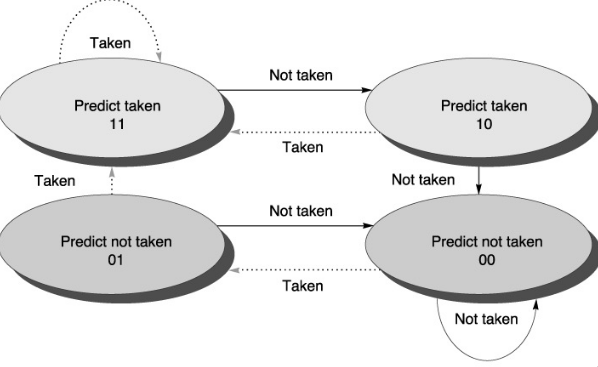
\includegraphics[scale=0.35]{02-ILP/2BP.png}
    \caption{Schema di predizione a due bit.}
\end{figure}

\nt{Questo schema è più complicato da implementare, ma funziona bene se il rapporto tra salti effettuati e non effettuati è molto sbilanciato. 

  Sistemi a più di 2 bit non aumentano di molto l'efficienza.
}

\clm{}{}{ 
  \begin{itemize}
    \item L'efficacia di questo schema dipende dal numero di entry nella memoria associativa che contiene i bit di predizione per le istruzioni di branch.
    \item Solitamente vengono usate cache da 4096 entry, sufficienti per la maggior parte delle istruzioni.
  \end{itemize}
}


\begin{figure}[!h]
    \centering
    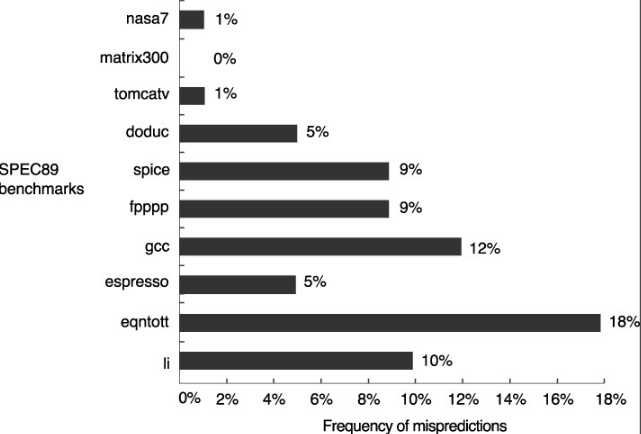
\includegraphics[scale=0.35]{02-ILP/2BP example.png}
    \caption{Percentuale di errori di predizione per banche prediction buffer a 2 bit e 4096 entry.}
\end{figure}

\nt{I processori moderni usano varianti di questa tecnica.}

\dfn{Schema a Predittori Correlati}{ 
  Uno \newfancyglitter{schema a predittori correlati} combina i predittori a due bit di due salti consecutivi, combinando così la storia locale di un salto con il comportamento dei salti circostanti.
}

\dfn{Schema a torneo}{ 
  Uno \newfancyglitter{schema a torneo} utilizza due predittori diversi per ciascun salto (uno a un bit, l'altro a due bit) e viene usato ogni volta quello che si è comportato meglio la volta precedente.
}

\nt{ 
Se il predittore dice che il salto va effettuato la CPU non può immediatamente iniziare la fase di fetch dell'istruzione puntata dal salto perché il suo indirizzo non è ancora noto e va calcolato (PC + offset specificato nell'istruzione di branch).
}

\dfn{Branch Prediction Cache}{ 
  Un \newfancyglitter{Branch Prediction Cache} (o Branch Prediction Buffer), per ogni controllo del branch, memorizza anche l'indirizzo a cui trasferire il controllo se il salto viene predetto come eseguito. Il valore PC + offset viene calcolato e messo nel buffer solo la prima volta che un branch viene eseguito.
} 

\begin{figure}[!h]
    \centering
    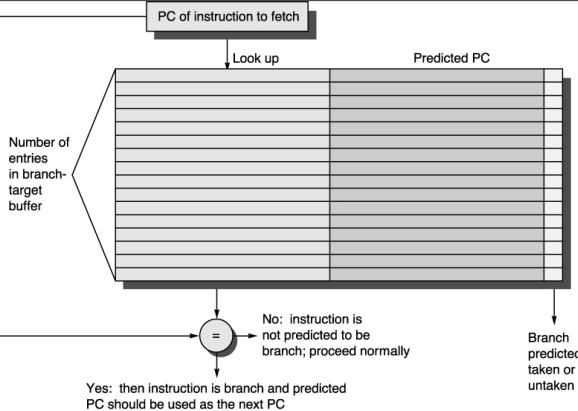
\includegraphics[scale=0.5]{02-ILP/BTB.png}
    \caption{Branch Prediction Buffer.}
\end{figure}

\subsubsection{Speculazione Hardware}

\dfn{Speculazione Hardware}{ 
  La \newfancyglitter{speculazione hardware} è la tecnica utilizzata nell'ILP dinamico per gestire e sfruttare vantaggiosamente situazioni in cui un dato non è presente in cache, ma deve essere recuperato dalla memoria primaria.
}

\cor{Istruzioni Speculative}{ 
Le istruzioni controllate dal branch vengono eseguite come se la predizione sul branch fosse corretta.
}

\nt{La speculazione hardware fa consumare corrente in più.} 

\cor{Unità di Commit}{ 
  Un insieme di entry interne alla CPU chiamato \fancyglitter{reorder buffer} (ROB) in cui vengono parcheggiate le istruzioni eseguite speculativamente, in attesa di sapere se dovessero essere effettivamente eseguite.
}

Quando il risultato di un'istruzione eseguita speculativamente è disponibile, viene inserito nel ROB e associato alla entry che contiene l'istruzione che lo ha prodotto. Le entry del ROB fungono da supporto alla ridenominazione dei registri. 
Quando la CPU sa che un'istruzione nel ROB doveva effettivamente essere eseguita ne esegue il commit: la toglie dal ROB e permette che il registro di destinazione dell'istruzione venga aggiornato. Se invece l'istruzione non doveva essere eseguita viene semplicemente rimossa da ROB.

\nt{L'esecuzione delle istruzioni può avvenire out-of-order, ma il commit deve avvenire nell'ordine in cui le istruzioni sono entrate nella CPU. Questo diminuisce la quantità di lavoro.}

\begin{figure}[!h]
    \centering
    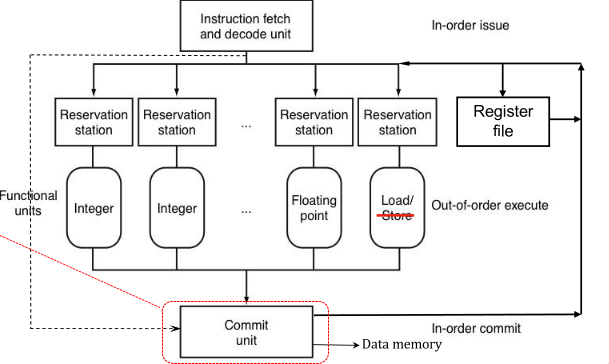
\includegraphics[scale=0.5]{02-ILP/Speculazione Hardware.png}
    \caption{Speculazione hardware.}
\end{figure}

\paragraph{Il ROB è composto da:} 

\begin{itemize}
  \item \fancyglitter{Il tipo di istruzione:} 
    \begin{itemize}
      \item \textit{Branch}, che non produce un risultato. 
      \item \textit{Store}, che scrive in RAM. 
      \item \textit{ALU o Load}, che scrivono in un registro.
    \end{itemize}
  \item \fancyglitter{Il campo di destinazione:} ossia il numero del registro o l'indirizzo della locazione di memoria modificati dall'istruzione, se questa riuscirà a passare la fase di commit. 
  \item \fancyglitter{Il campo valore:} memorizza temporaneamente il risultato dell'esecuzione dell'istruzione fino al commit. 
  \item \fancyglitter{Il campo ready:} indica che l'istruzione ha terminato l'esecuzione e il contenuto del campo valore è valido.
\end{itemize}

\paragraph{Con la speculazione si hanno 4 macropassi:}

\begin{enumerate}
  \item \fancyglitter{Issue:} dopo le fasi IF e ID, l’istruzione I viene avviata ad una entry di
una stazione di prenotazione. \textit{I viene anche inserita in fondo
al ROB, facendo scalare verso la cima tutte le istruzioni già
presenti nel ROB.} Se disponibili, gli operandi di I vengono inviati alla entry che
contiene I, prelevandoli da uno dei registri, da un’altra stazione
di prenotazione, \textit{o da una entry del ROB}. 

\textit{Il numero della entry del ROB che contiene I viene scritto
nella stazione di prenotazione di I} (così alla fine della fase EX
di I, il risultato di I potrà essere inviato a quella entry del ROB).

  \item \fancyglitter{Execute:} quando gli operandi sono tutti disponibili l’istruzione I viene
inoltrata all’Unità Funzionale corrispondente. 

\item \fancyglitter{Write Result:} quando il risultato di I è pronto, viene scritto sul CDB, e da qui
viene inoltrato ad ogni stazione di prenotazione che lo stava
aspettando (ma, notate, non nel register file o in RAM).
  
\textit{Il risultato di I viene anche inoltrato verso il ROB e scritto
nel campo valore della entry che contiene una copia
dell’istruzione I} (il numero della entry del ROB da usare è
quello associato ad I durante la fase Issue).

\item \fancyglitter{Commit:} quando una istruzione nel ROB raggiunge la cima della coda
(perché altre istruzioni sono state inserite in fondo alla coda), il
commit può avvenire. Se: 
\begin{itemize}
  \item L’istruzione non è un branch, il contenuto del campo valore
è trasferito nel registro o nella locazione di RAM opportuni.
L’istruzione viene rimossa dal ROB. 
\item L’istruzione è un branch con predizione sbagliata, tutto
il ROB viene svuotato, e la computazione è riavviata
dall’istruzione corretta.
\end{itemize}
\end{enumerate}

\subsection{Multiple Issue con ILP Dinamico}

Se alle tecniche già accennate sull'ILP dinamico si aggiunge il multiple issue si ha la descrizione della maggior parte dei processori moderni (single core). Il numero di istruzioni lanciate in parallelo dal multiple issue è anch'esso dinamico: varia a ogni ciclo di clock. 

\paragraph{Il multiple issue richiede:} 

\begin{itemize}
  \item Un numero sufficiente di unità funzionali
per l’esecuzione di più istruzioni in parallelo. Per esempio, più
ALU, più unità di moltiplicazione intera / Floating Point, e così via.
\item Possibilità di prelevare dalla Instruction Memory più
istruzioni, e dalla Data Memory più operandi, per ciclo di clock. 
\item Possibilità di indirizzare in parallelo più registri della CPU,
e deve essere possibile leggere e/o scrivere i registri usati da diverse
istruzioni in esecuzione nello stesso ciclo di clock.
\end{itemize}

\nt{Un Processore con tutte queste caratteristiche è detto processore superscalare.} 

\subsubsection{Funzionamento di un Processore Superscalare:}

\begin{enumerate}
  \item Preleva dalla IM (cache di primo livello) N istruzioni per ciclo di clock, dove N è il numero di istruzioni che la IM riesce a fornire in parallelo. 
  \item Le istruzioni vengono messe in una Instruction queue (IQ) per poter essere analizzate dalla logica della CU che deve controllare la presenza di eventuali dipendenze. 
  \item Una volta analizzate le istruzioni nella IQ, vengono avviate
all’esecuzione, cioè instradate verso le stazioni di prenotazione, alcune delle istruzioni indipendenti, liberando così spazio nella
Instruction Queue. 
\item Al successivo ciclo di clock viene prelevato dalla IM un altro
gruppo N di istruzioni. 
\item A regime quindi, la IQ tende riempirsi di istruzioni, e se ad un certo
ciclo di clock M istruzioni vengono avviate all’esecuzione, al
massimo M $\leq$ N altre istruzioni possono essere prelevate dalla IM al
successivo ciclo di clock.
\item Se la IQ è piena, e a causa delle dipendenze
nessuna istruzione è stata inviata alla fase EXECUTE al ciclo
precedente, nessuna istruzione potrà essere prelevata dalla IM
al ciclo successivo. 

\end{enumerate}

\clm{}{}{ 
\begin{itemize}
  \item A regime, la CPU deve controllare la presenza
di dipendenze tra qualche decina di istruzioni, il che può richiedere
migliaia di confronti incrociati, che devono essere fatti in uno o due
cicli di clock. 
\item Se è implementata la speculazione hardware la
CPU deve anche essere in grado di eseguire il commit di più
istruzioni nel ROB per ciclo di clock, che altrimenti diviene il collo
di bottiglia del sistema.
\end{itemize}
} 

\qs{}{Perché ILP dinamico funziona?} 

\begin{itemize}
  \item I miss cache non sono prevedibili staticamente, e l’ILP dinamico
può parzialmente nasconderli eseguendo altre istruzioni, mentre una
istruzione attende dalla RAM il dato mancante in cache.  
\item I branch non sono prevedibili con accuratezza in modo statico
e il BP dinamico e la speculazione aumentano la probabilità di
riuscire a sbrigare del lavoro utile in anticipo rispetto al momento
in cui si conosce l’esito dell’esecuzione delle istruzioni di branch. 
\item L’ILP statico funziona bene solo su una specifica architettura. Invece,
con l’ILP dinamico i programmi possono essere eseguiti su
architetture diverse (purché con ISA compatibili) per numero di
unità funzionali, numero di registri rinominabili, numero di stage
della pipeline, tipo di predizione dei branch (processori Intel e
AMD).
\end{itemize}

\subsubsection{Limiti Teorici dell'ILP Dinamico}

Tutte le limitazioni, a eccezione delle true data dependence, possono essere eliminate se si ha hardware sufficientemente potente. Si possono fare le seguenti assunzioni: 

\begin{itemize}
  \item \fancyglitter{Register Renaming:} la CPU ha un numero infinito di registri rinominabili. 
  \item \fancyglitter{Branch Prediction:} perfetta. 
  \item \fancyglitter{Memory-Address alias analysis:} tutti gli indirizzi di RAM sono noti, per cui si possono sempre evitare le dipendenze sui nomi in RAM.
\item \fancyglitter{Multiple Issue:} illimitato. 
\item \fancyglitter{Cache Memory:} non si verificano miss.
\end{itemize}

\begin{figure}[!h]
    \centering
    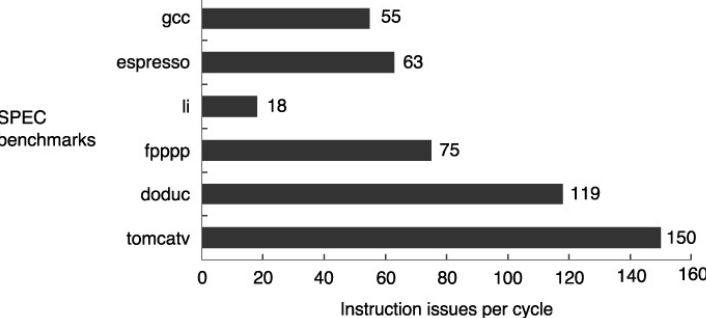
\includegraphics[scale=0.5]{02-ILP/limiti teorici.png}
    \caption{Alcuni Benchmark.}
\end{figure}

Ritornando a un processore più realistico si limita il numero massimo di istruzioni consecutive che possono essere contemporaneamente prese in considerazione per cercare dipendenze sui dati.

\begin{figure}[!h]
    \centering
    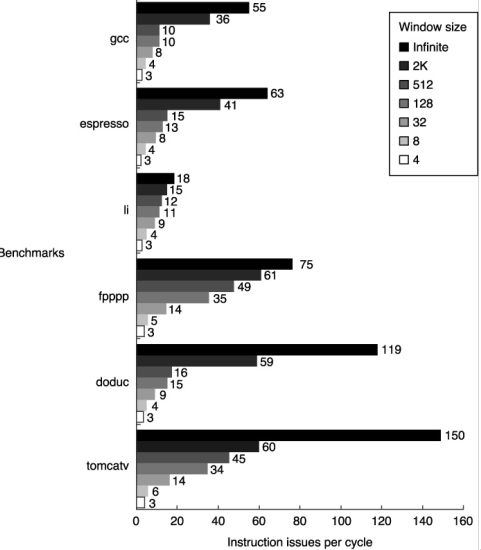
\includegraphics[scale=0.5]{02-ILP/limiti 2.png}
    \caption{Alcuni Benchmark con la limitazione sul multiple issue.}
\end{figure}

Successivamente possiamo introdurre la possibilità di errore nella branch prediction. 

\begin{figure}[!h]
    \centering
    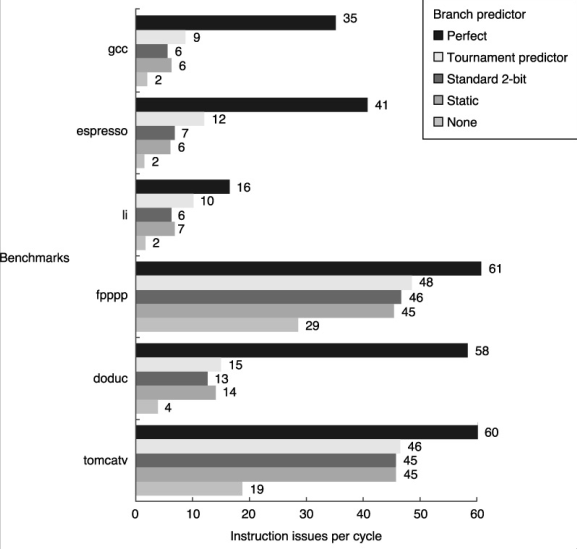
\includegraphics[scale=0.5]{02-ILP/limiti 3.png}
    \caption{Alcuni Benchmark con la limitazione sul multiple issue (con 2k istruzioni) e sulla branch prediction.}
\end{figure}

\nt{Aggiungendo anche tutte le altre limitazioni le performance calano drasticamente. 
I progettisti sono ormai convinti che i processori moderni abbiano
già da alcuni anni raggiunto il massimo livello possibile di
sfruttamento dell’ILP, e che ulteriori migliorie possano venire solo
da avanzamenti tecnologici.
}



\section{ILP Statico} 

















